\documentclass[../notes.tex]{subfiles}

\pagestyle{main}
\renewcommand{\chaptermark}[1]{\markboth{\chaptername\ \thechapter\ (#1)}{}}

\begin{document}




\chapter{Introduction}
\section{Introduction}
\begin{itemize}
    \item \marginnote{9/5:}Normally, only about 20 kids enroll in this class per year. This year, there are 40.
    \begin{itemize}
        \item This is a typical class for the first-year grad students in OChem, but Elkin asks what made advanced undergrads and second-year grad students enroll, as well as just so many of us overall.
        \item Radosevich told all the inorganic kiddos to take this class!
        \item Bioinorganic and Organometallics also aren't being offered because everyone's on sabbatical.
    \end{itemize}
    \item Oleta Johnson came to sit in on Masha's class! Oleta is Masha's "best friend."
    \item The lecture now begins (on MIT Time).
    \item Masha will teach the first half of the course; Alex will teach the second half.
    \begin{itemize}
        \item TF is Jonathan Edward, an Elkin kiddo.
        \begin{itemize}
            \item He will hold weekly OH, study sessions, grades problems and exams, etc.
            \item Has a mastery of the subject material (took 5.53 last year), and unrivaled "approachability."
        \end{itemize}
        \item Reach out to Masha or Alex if we have issues with the subject material, our own journeys in grad school or undergrad, etc. It's easier to fix problems early in the semester!
    \end{itemize}
    \item Overview of the course.
    \begin{itemize}
        \item 1st half.
        \begin{itemize}
            \item Basically physical organic chemistry.
            \item A deep dive on structure and reactivity.
        \end{itemize}
        \item 2nd half.
        \begin{itemize}
            \item Basically reaction mechanisms.
            \item Kinetics, rate laws, kinetic isotope effects (KIEs), methodology experiments, etc.
        \end{itemize}
        \item The tools presented herein are broadly applicable to various fields of chemistry.
    \end{itemize}
    \item This course will teach us to\dots
    \begin{itemize}
        \item Propose \emph{reasonable} mechanisms for organic reactions;
        \item Scrutinize mechanisms in the literature;
        \begin{itemize}
            \item That is, figure out if a proposed mechanism is reasonable or not, evaluate the authors' evidence, and identify follow-up experiments that can be run.
        \end{itemize}
        \item Design experiments to distinguish and test proposed mechanisms;
        \item Conduct our own mechanistic study.
    \end{itemize}
    \pagebreak
    \item Masha gives the metacognition spiel again.
    \begin{itemize}
        \item Know our strengths and weaknesses (correct these by reviewing undergrad notes and Googling).
    \end{itemize}
    \item Course logistics.
    \begin{itemize}
        \item 2 exams.
        \begin{itemize}
            \item Fully online; they are trusting us to work alone on the honor system.
        \end{itemize}
        \item 4 problem sets.
        \begin{itemize}
            \item Posted 1 week before they are due.
            \item Encouraged to work collaboratively, but submit our own work.
            \item Jonathan and Masha will reserve a study room in which we can collaborate.
        \end{itemize}
        \item 1 mechanistic proposal.
        \begin{itemize}
            \item Engage the literature!
        \end{itemize}
        \item Textbook: \textcite{bib:Anslyn}.
        \begin{itemize}
            \item The standard textbook for PhysOrg (do readings and practice problems as needed).
            \item Jonathan is working on a correspondence of lectures to chapters.
        \end{itemize}
        \item Reach out to Masha, Alex, or Jonathan if we have any questions!
        \begin{itemize}
            \item If you ever miss class, post a new topic on the Canvas discussion board asking for notes (and be generous in uploading your own).
        \end{itemize}
    \end{itemize}
    \item We now begin the course content.
    \item \textbf{Mechanism}: An accounting of all bond-making and bond-breaking events in a reasonable sequence.
    \begin{itemize}
        \item Mechanisms don't exist in the physical sense; it is more of a \emph{model} of how things proceed.
    \end{itemize}
    \item Mechanisms exist in four levels of depth.
    \begin{enumerate}
        \item Describe electron movement via arrow pushing.
        \begin{figure}[h!]
            \centering
            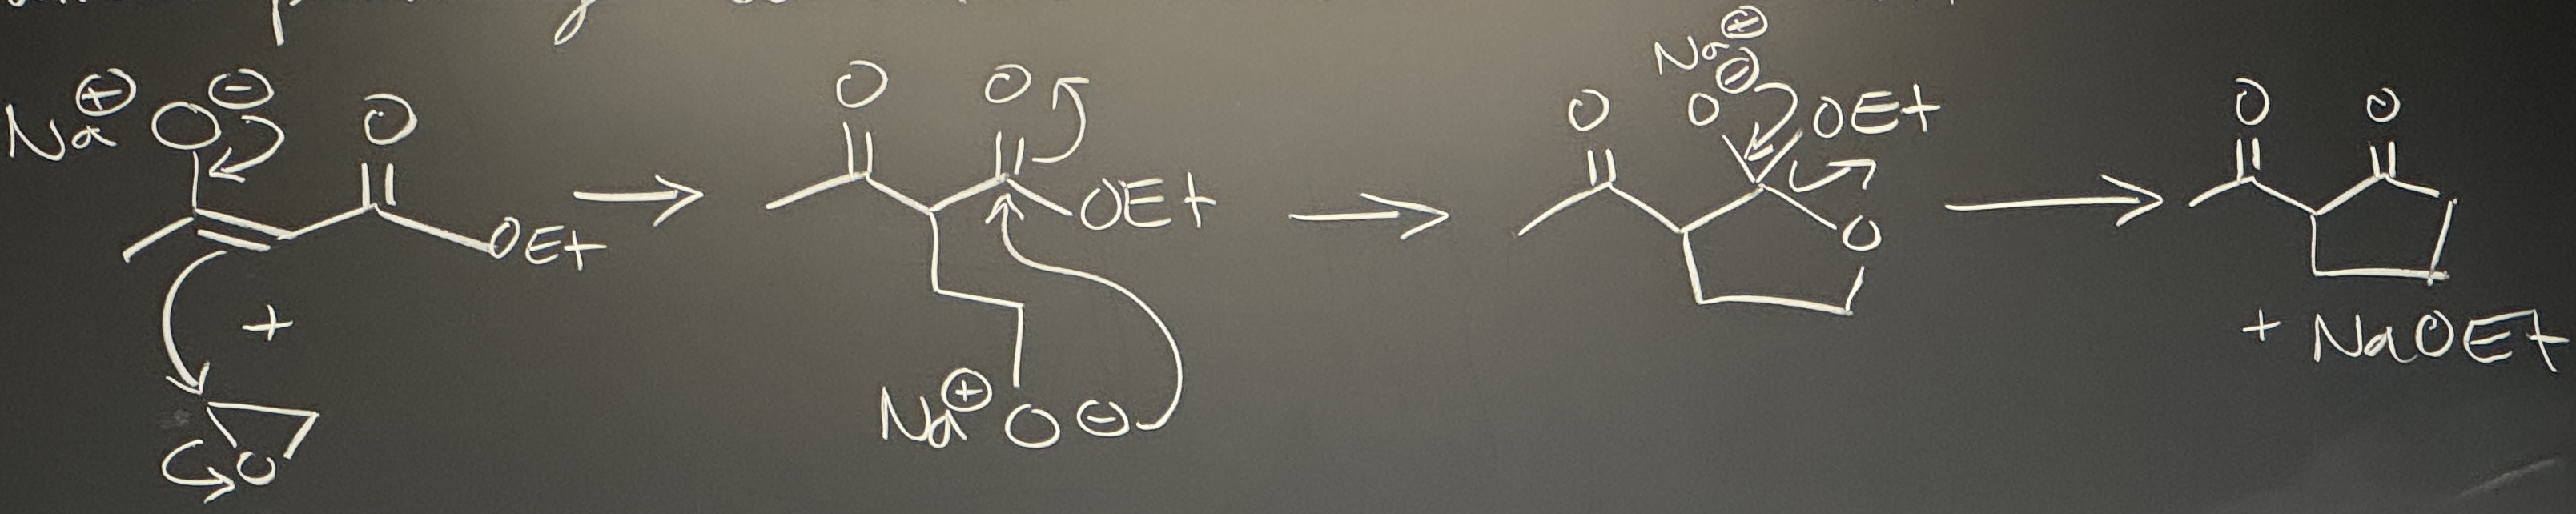
\includegraphics[width=0.7\linewidth]{mechDepth1.JPG}
            \caption{Mechanism depth level 1 (arrow pushing).}
            \label{fig:mechDepth1}
        \end{figure}
        \begin{itemize}
            \item Equivalent level: 5.47 \& undergrad organic.
            \item Example: Figure \ref{fig:mechDepth1}.
            \begin{itemize}
                \item In every step that we push arrows, we start at a region of high electron density, we make and break sequential bonds, and we leave the negative charge on an electronegative atom.
                \item Once we have completed one step, we can start again from a new region of high electron density, making and breaking bonds, and drawing the product.
                \item We repeat this process again and again until we reach the final product.
                \item Arrow pushing conserves net neutral charges on molecules.
            \end{itemize}
            \item Aside: Arrow types.
            \begin{figure}[H]
                \centering
                \footnotesize
                \begin{subfigure}[b]{0.1\linewidth}
                    \centering
                    \schemestart
                        \chemfig{@{a}-[,,,,opacity=0]@{b}}
                    \schemestop
                    \chemmove{
                        \draw [curved arrow={0pt}{0pt}] (a) to[bend left=60,looseness=1.5] (b);
                    }
                    \caption{$2\e[-]$.}
                    \label{fig:arrowTypesa}
                \end{subfigure}
                \begin{subfigure}[b]{0.12\linewidth}
                    \centering
                    \schemestart
                        \chemfig{@{a}-[,,,,opacity=0]@{b}}
                    \schemestop
                    \chemmove{
                        \draw [curved arrow={0pt}{0pt},arrows={-Stealth[harpoon,flex]}] (a) to[bend left=60,looseness=1.5] (b);
                    }
                    \caption{$1\e[-]$.}
                    \label{fig:arrowTypesb}
                \end{subfigure}
                \begin{subfigure}[b]{0.16\linewidth}
                    \centering
                    \schemestart\arrow{<=>}\schemestop
                    \caption{Equilibrium.}
                    \label{fig:arrowTypesc}
                \end{subfigure}
                \begin{subfigure}[b]{0.16\linewidth}
                    \centering
                    \schemestart
                        \chemleft[
                            \subscheme{
                                \chemfig{A}
                                \arrow{<->}
                                \chemfig{B}
                            }
                        \chemright]
                    \schemestop
                    \caption{Resonance.}
                    \label{fig:arrowTypesd}
                \end{subfigure}
                \begin{subfigure}[b]{0.2\linewidth}
                    \centering
                    \schemestart\arrow{=retro>}\schemestop
                    \caption{Retrosynthetic.}
                    \label{fig:arrowTypese}
                \end{subfigure}
                \caption{Arrow types in arrow pushing.}
                \label{fig:arrowTypes}
            \end{figure}
            % \begin{itemize}
            %     \item Double-headed arrows: 2 electrons.
            %     \item Single-headed arrows: 1 electron.
            %     \item Equilibrium arrows.
            %     \item Resonance arrows.
            %     \item Retrosynthetic arrows.
            % \end{itemize}
        \end{itemize}
        \item Determine the transition-state structures.
        \begin{figure}[H]
            \centering
            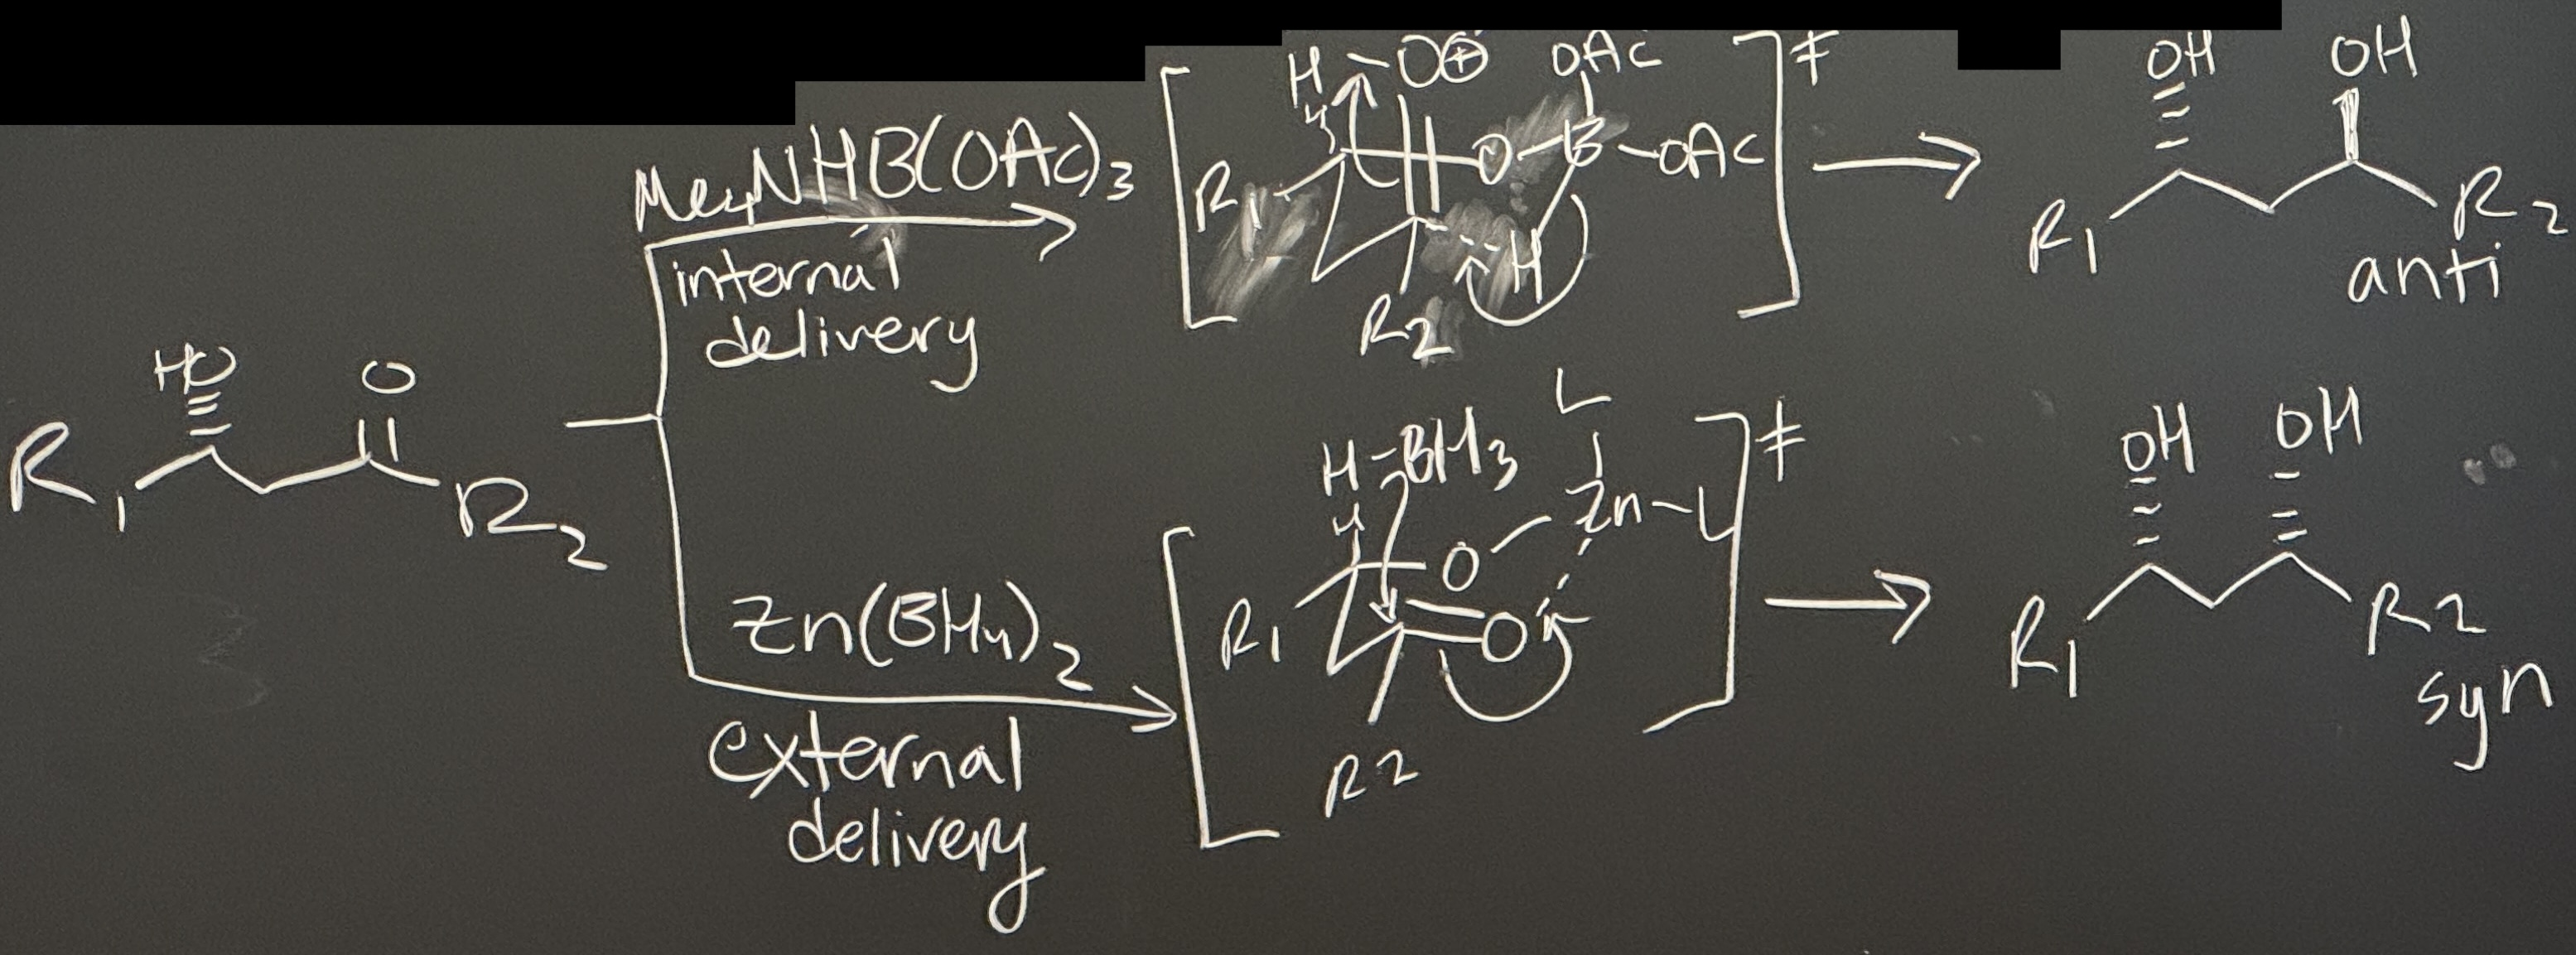
\includegraphics[width=0.6\linewidth]{mechDepth2.JPG}
            \caption{Mechanism depth level 2 (transition states).}
            \label{fig:mechDepth2}
        \end{figure}
        \begin{itemize}
            \item Equivalent level: 5.47 \& undergrad organic, as well.
            \item Can't observe these directly --- infer from observed selectivities (stereo-, regio-, etc.).
            \item Example: Figure \ref{fig:mechDepth2}.
            \begin{itemize}
                \item Reacting a $\beta$-ketol with two different reducing agents. We can infer the structure of the transition state from the stereochemistry of the product.
                \item Internal delivery of tetramethylammonium triacetoxyborohydride yields an \emph{anti}-diol.
                \item External delivery of zinc borohydride yields a \emph{syn}-diol.
            \end{itemize}
            \item Takeaway: We know that in organic chemistry, transition states should have chair-like structures for stability.
            \begin{itemize}
                \item Since we see chair like structures in Figure \ref{fig:mechDepth2}, we can infer that these mechanisms are reasonable. Indeed, they have stood for decades!
            \end{itemize}
        \end{itemize}
        \item Determine the energy landscape and the full reaction coordinate.
        \begin{figure}[h!]
            \centering
            \begin{subfigure}[b]{\linewidth}
                \centering
                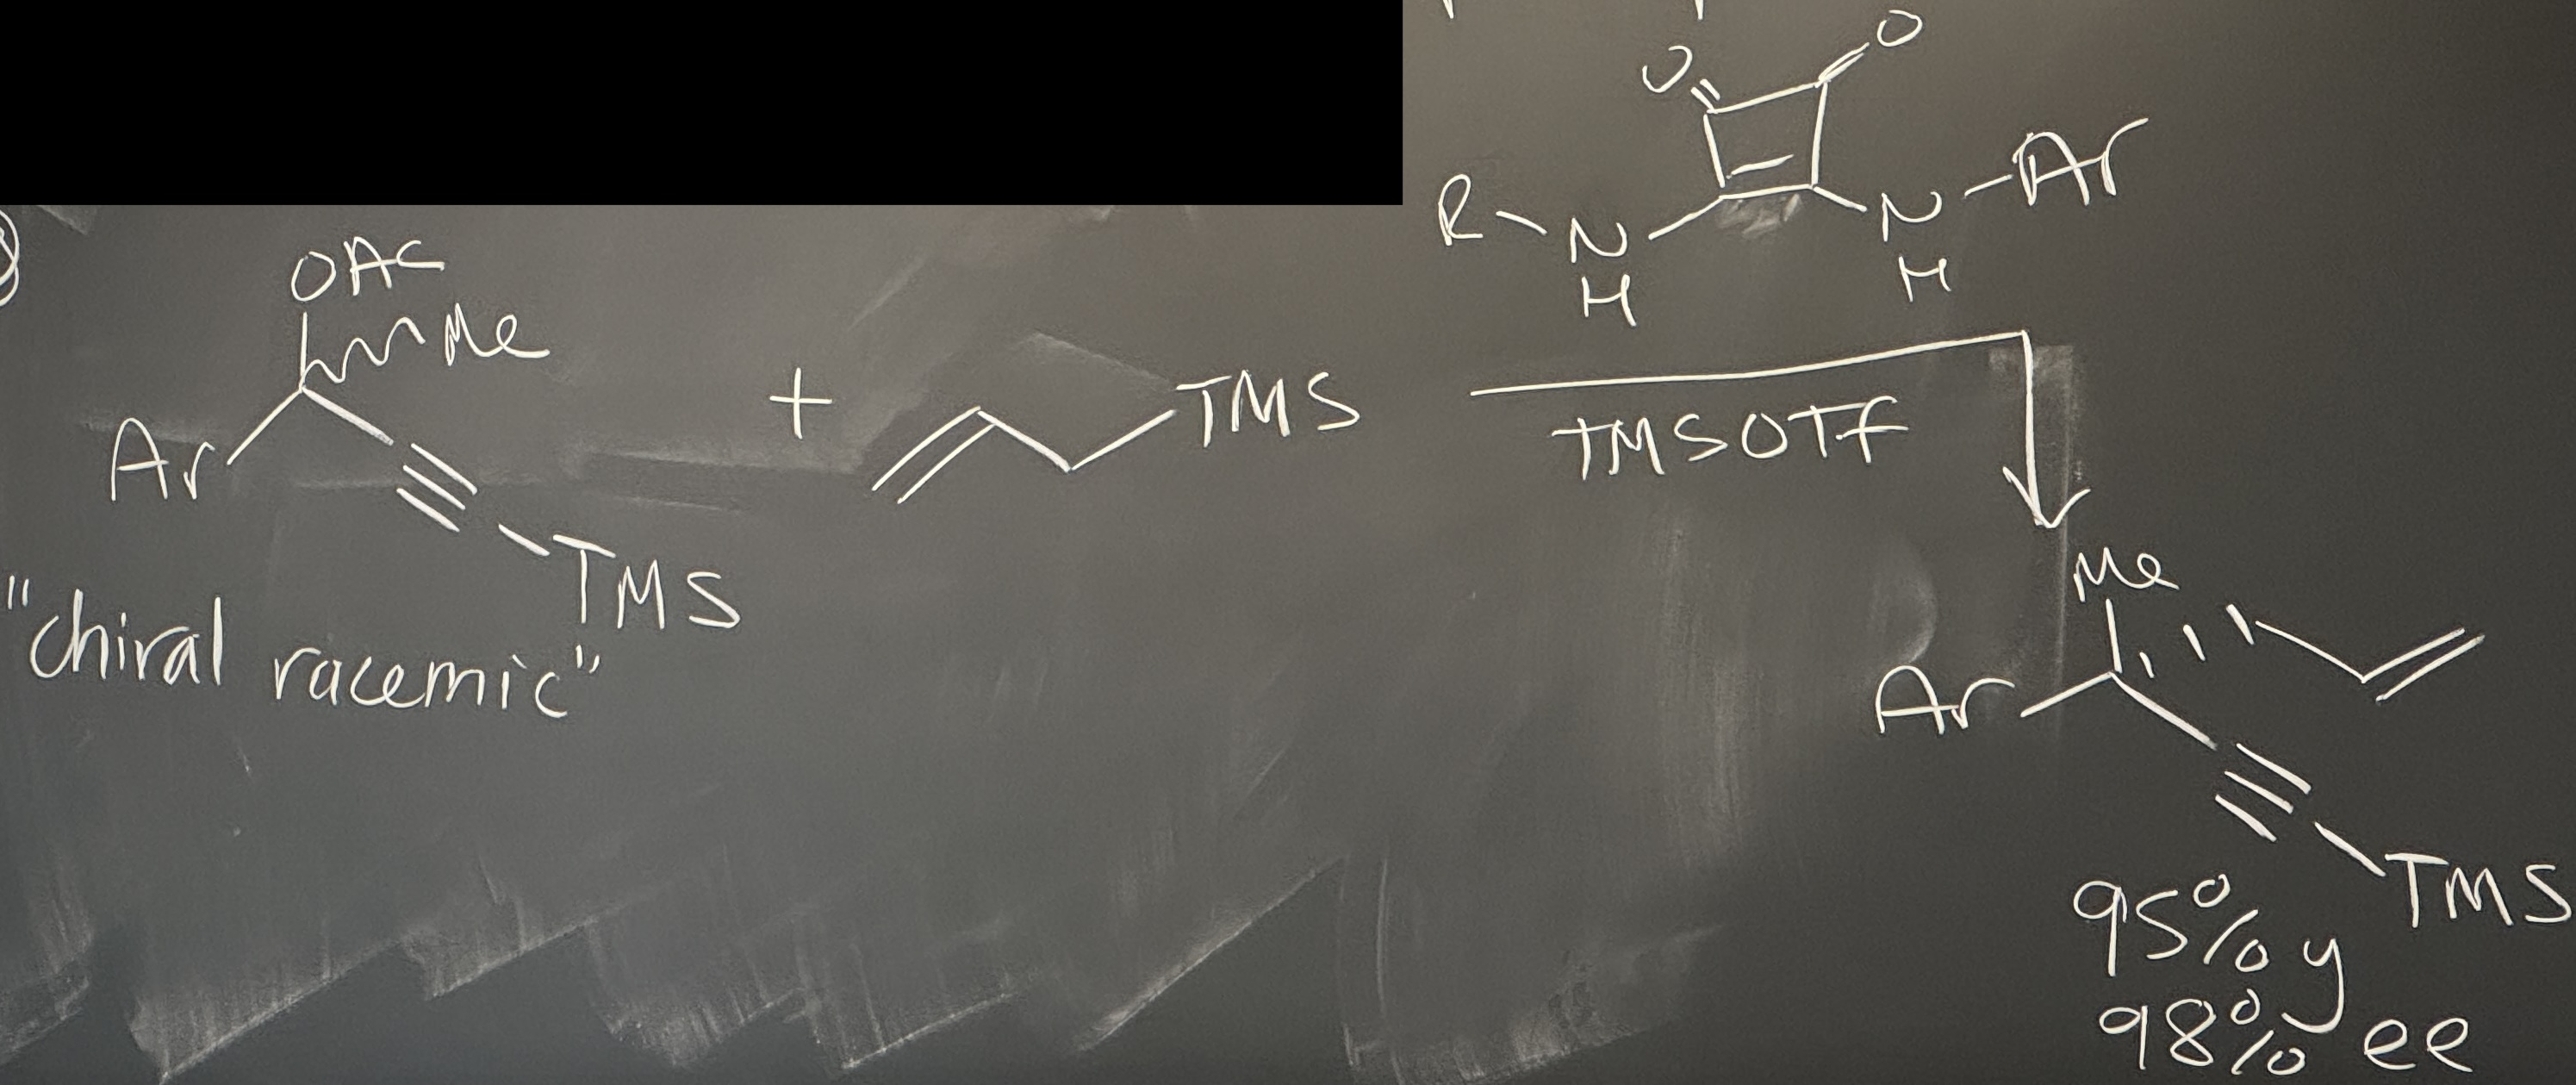
\includegraphics[width=0.5\linewidth]{mechDepth3a.JPG}
                \caption{A reaction.}
                \label{fig:mechDepth3a}
            \end{subfigure}\\[1em]
            \begin{subfigure}[b]{\linewidth}
                \centering
                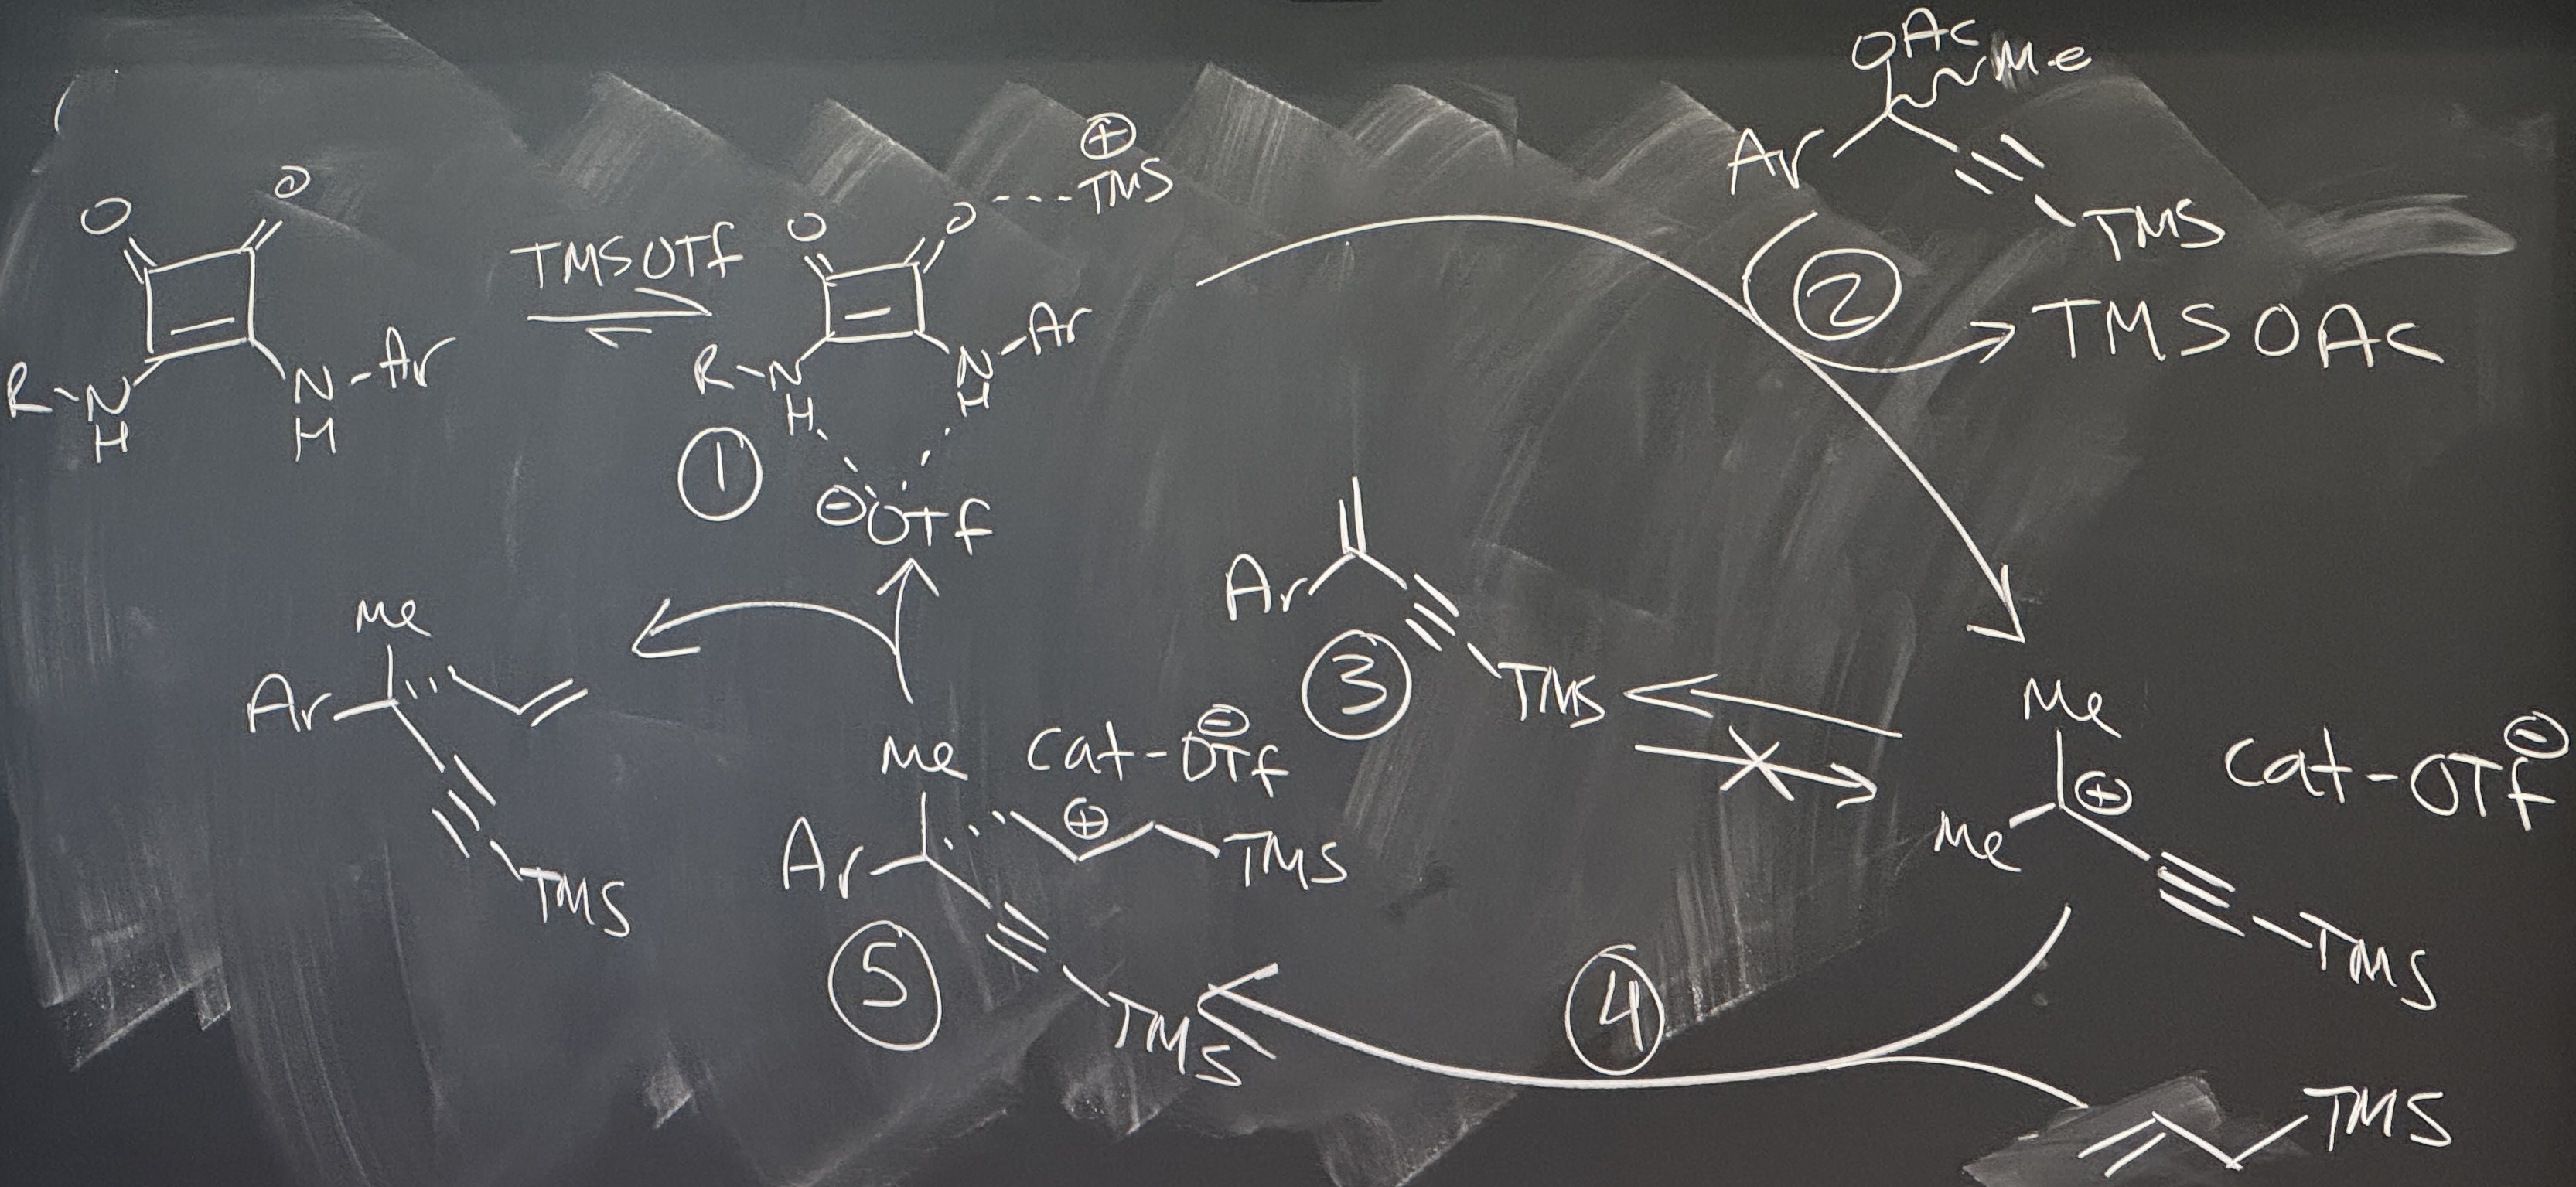
\includegraphics[width=0.65\linewidth]{mechDepth3b.JPG}
                \caption{The full reaction coordinate.}
                \label{fig:mechDepth3b}
            \end{subfigure}
            \caption{Mechanism depth level 3 (full reaction coordinate).}
            \label{fig:mechDepth3}
        \end{figure}
        \pagebreak
        \begin{itemize}
            \item Equivalent level: This class!
            \item This level of analysis enables us to\dots
            \begin{itemize}
                \item Rationally design experiments that improve the reaction (i.e., conduct methods development and catalysis);
                \item Discover new mechanistic principles.
            \end{itemize}
            \item Example: Figure \ref{fig:mechDepth3}.
            \begin{itemize}
                \item Figure \ref{fig:mechDepth3a} depicts a curious reaction: Propargyl acetate (with racemic chirality) reacts with an allyl silane under a squaramide catalyst and TMSOTf (a Lewis acid).
                \item Even though the starting material is racemic, we get an enantioenriched allylated propargyl acetate (95\% yield, 98\% ee) as a product.
            \end{itemize}
            \item The mechanism (Figure \ref{fig:mechDepth3b}) proceeds in five steps.
            \begin{enumerate}[label={(\arabic*)}]
                \item Activate the catalyst to form an intermediate.
                \item Engage the starting material to form a tertiary carbocation.
                \item This carbocation can off-cycle to form an elimination product.
                \item Preferably, however, we engage our nucleophile (the allyl silane) to get a new cationic adduct, counterbalanced by the catalyst-triflate complex.
                \item The adduct goes on to eliminate our product and regenerate the starting intermediate.
            \end{enumerate}
            \item This mechanism originated from a beautiful mechanistic study by this paper's authors. Let's discuss some of their insights.
            \begin{enumerate}[label={(\arabic*)}]
                \item This complex is the \textbf{resting state}.
                \begin{itemize}
                    \item Analytical technique(s): Binding experiments between the catalyst and \ce{TMSOTf}.
                    \item This is a thermodynamic insight.
                \end{itemize}
                \item This step is the \textbf{rate-determining step}.
                \begin{itemize}
                    \item Analytical technique(s): The rate law (a kinetic parameter) and \textbf{Hammett plots}.
                \end{itemize}
                \item This step is an irreversible side reaction.
                \begin{itemize}
                    \item Analytical technique(s): Competition experiments.
                    \item Since this step is post-RDS in the mechanism, it is quite difficult to study.
                    \item Takeaway: It is easy to see things between the resting state and RDS, but everything after the RDS is like magic. These steps are very hard --- but very important --- to probe. Indeed, knowing how and where side reactions originate provides clues on how to stop them!
                \end{itemize}
                \item This step is the \textbf{stereo-determining step}.
                \begin{itemize}
                    \item Analytical technique(s): The kinetic isotope effect (review this from CHEM 20200!!).\footnote{KIEs should probably be used in our end-of-class mechanistic proposal, will likely be used in our research, and \emph{can} probe post-RDS steps.}
                    \begin{itemize}
                        \item Revealed that stereoinduction was due to noncovalent interaction (NCIs) between the catalyst and intermediate.
                    \end{itemize}
                    \item Usually, your stereo-determining step is your RDS, but not in this regime. It is very hard to optimize a post-RDS, stereo-determining step.
                \end{itemize}
                \item This intermediate is stabilized due to hyperconjugation from silicon.
                \begin{itemize}
                    \item Analytical technique(s): $\beta$-silicon effects and $\alpha$-silicon effects.
                \end{itemize}
            \end{enumerate}
            \item We will learn all of the techniques mentioned above in this class.
            \item Impact of this paper.
            \begin{itemize}
                \item It's one of the first enantioselective S\textsubscript{N}1 reactions.
                \item It has a decoupled RDS and stereo-determining step, but gets high ee regardless.
                \begin{itemize}
                    \item This was an unprecedented result, and it changed the way we as chemists think about optimizing entantioselective reactions.
                \end{itemize}
                \item Reference: \textcite{bib:WendlandtMechanism}.
            \end{itemize}
        \end{itemize}
        \pagebreak
        \item Computationally determine the entire multidimensional energy surface.
        \begin{figure}[h!]
            \centering
            \footnotesize
            \schemestart
                \chemfig{Ph-[:60]=_-[:-60]Ph}
                \arrow{->[$h\nu$]}
                \chemfig{Ph-[:60]=_-[:60]Ph}
            \schemestop
            \caption{Mechanism depth level 4 (full energy manifold).}
            \label{fig:mechDepth4}
        \end{figure}
        \begin{itemize}
            \item Currently only possible for very simple systems.
            \item Example: Figure \ref{fig:mechDepth4}.
            \begin{itemize}
                \item This is a transformation under light from a \emph{cis}-olefin to a \emph{trans}-olefin.
                \item The authors tracked the reaction with femtosecond (\num{e-15}) Raman spectroscopy.
                \item Reference: \textcite{bib:computational}.
            \end{itemize}
            \item Full computational modeling is a pipe dream that would hugely enable our work as chemists.
        \end{itemize}
    \end{enumerate}
    \item \textbf{Resting state} (of a catalyst): The state of a catalyst such that if you took an NMR of the reaction mixture at any given time, 95\% of the sample would look like this.
    \item \textbf{Rate-determining step}. \emph{Also known as} \textbf{rate-limiting step}.
    \begin{itemize}
        \item Important because if you can speed it up, you can speed up the whole thing!
    \end{itemize}
    \item \textbf{Rate law}: A measure of how the rate of reaction is influenced by the concentration of different components.
    \item \textbf{Hammett plot}: A mechanistic tool to probe what the rate-determining step is.
    \item \textbf{Stereo-determining step}: The step in a reaction mechanism that sets the stereochemistry of the final product; the ee of this step is the ee of the product.
    \item Takeaway: Keep in mind these various levels when we're trying to work out a reaction!
    \item Online tool: Reference Resolver!!
    \begin{itemize}
        \item Give it the journal, year, and page number, and it brings us to the article.
        \item There is a website, but also a browser plugin worth getting.
    \end{itemize}
    \item Now that we've discussed the kinds of mechanisms, let's talk about what a mechanism can and can't do for us.
    \item A mechanism \emph{can} tell us\dots
    \begin{itemize}
        \item Thermodynamics and equilibria: Identity and structure of the ground state species;
        \item Kinetics: Identity and structure of the transition state (TS) structures \emph{relative} to the ground state structures;
        \begin{itemize}
            \item We can't identify anything about the transition state in absolutes, but we can take educated guesses about intermediates and infer their approximate form.
        \end{itemize}
        \item Intermediates: Evidence of reaction intermediates;
        \begin{itemize}
            \item Example: The tetrahedral intermediate.
            \item Such intermediates are often called \textbf{metastable}.
        \end{itemize}
        \item RDS: Insight into selectivity and RDS's.
    \end{itemize}
    \item \textbf{Metastable} (state): An intermediate energetic state within a dynamical system other than the system's state of least energy. \emph{Also known as} \textbf{unstable equilibrium}.
    \begin{itemize}
        \item A rectangular prism standing on its end under the force of gravity is metastable.
    \end{itemize}
    \item A mechanism \emph{cannot} be proven.
    \begin{itemize}
        \item Mechanisms are hypotheses or proposals that can only be \emph{disproven} or \emph{supported}.
        \item This is because experimental data often fits several possible mechanisms; there might be a hidden secret mechanism that we never thought of.
        % \item We can only say, "here's a mechanism that's consistent with the data and allows me to make useful predictions."
        \item In sum, a mechanism is an interpretation that is consistent with \emph{all} the data.
        \begin{itemize}
            \item If a mechanism doesn't fit our data (even a little bit), either our mechanism is missing something (maybe a little something) or our experiment is flawed (and we need to rerun it or run something else).
        \end{itemize}
    \end{itemize}
    \item Best practices.
    \begin{itemize}
        \item The best mechanisms provide \emph{testable} predictions.
        \begin{itemize}
            \item If a mechanism doesn't provide testable predictions, it is not a useful model.
            \item If it's not useful, it's not grounded in good scientific practice.
        \end{itemize}
        \item The best experiments disprove a mechanistic proposal.
        \begin{itemize}
            \item In practice, we list all possible mechanisms and try to disprove them with experiments.
            \item When we submit to a journal, we do not say that our mechanism is proven, but we state our reasoning and our reviewers try to think of other mechanisms that could fit the data.
        \end{itemize}
    \end{itemize}
    \item Aside: Both Alex and Masha care about how scientists actually do science and how science can be done ethically.
    \begin{itemize}
        \item They want this to be a practical class that would enable us to go in the lab and run any of these experiments.
    \end{itemize}
    \item We study mechanisms to\dots
    \begin{itemize}
        \item Ensure a safe, robust (reproducible), and scalable process;
        \begin{itemize}
            \item This is especially important in process chemistry.
            \item Human consequences of failing at safety, scale, and/or robustness:
            \begin{itemize}
                \item Your ammonia plant could explode; it is essential to watch any runaway exotherms in a mechanism and control them!
                \item Your drug might not make it to market if its synthesis can't be scaled up.
            \end{itemize}
        \end{itemize}
        \item Improve reaction features such as yield, selectivity, and greenness;
        \item Expand scope and enable predictability;
        \begin{itemize}
            \item Think about reactions we run daily, such as the Suzuki coupling. It always works, and it's easily applicable in a wide range of settings \emph{because} we understand the mechanism.
        \end{itemize}
        \item Understand systems on a molecular level.
        \begin{itemize}
            % \item Because \emph{chemists manipulate matter} on a molecular level.
            \item Masha takes 30 seconds to preach about how mechanisms are critically important knowledge that will be passed down the generations.
        \end{itemize}
    \end{itemize}
    \item Aspects of mechanism: Consider the S\textsubscript{N}2 reaction, \ce{Br- + Me-I -> Br-Me + I-}.
    \begin{figure}[H]
        \centering
        \footnotesize
        \begin{subfigure}[b]{0.3\linewidth}
            \centering
            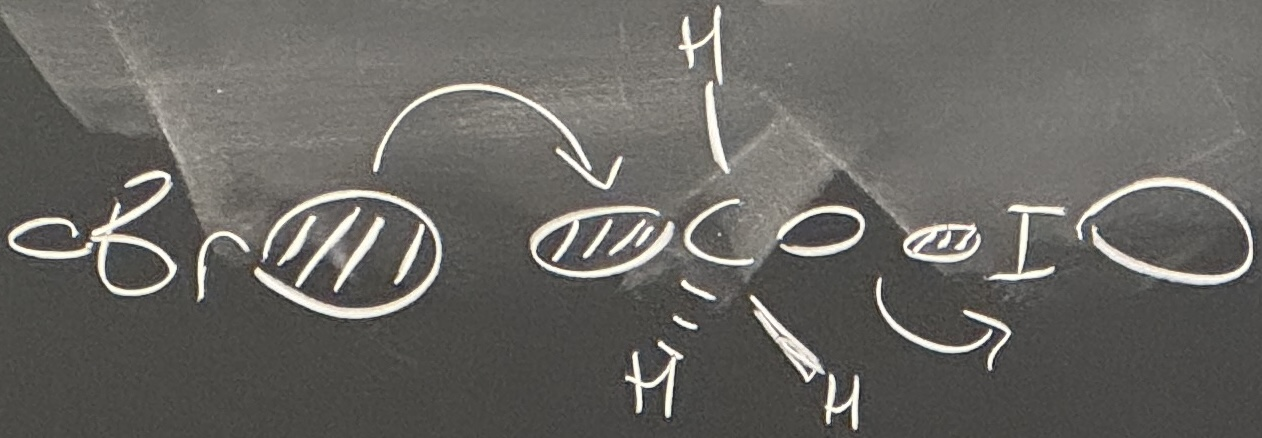
\includegraphics[width=0.7\linewidth]{mechAspectsa.JPG}
            \caption{Orbitals.}
            \label{fig:mechAspectsa}
        \end{subfigure}
        \begin{subfigure}[b]{0.3\linewidth}
            \centering
            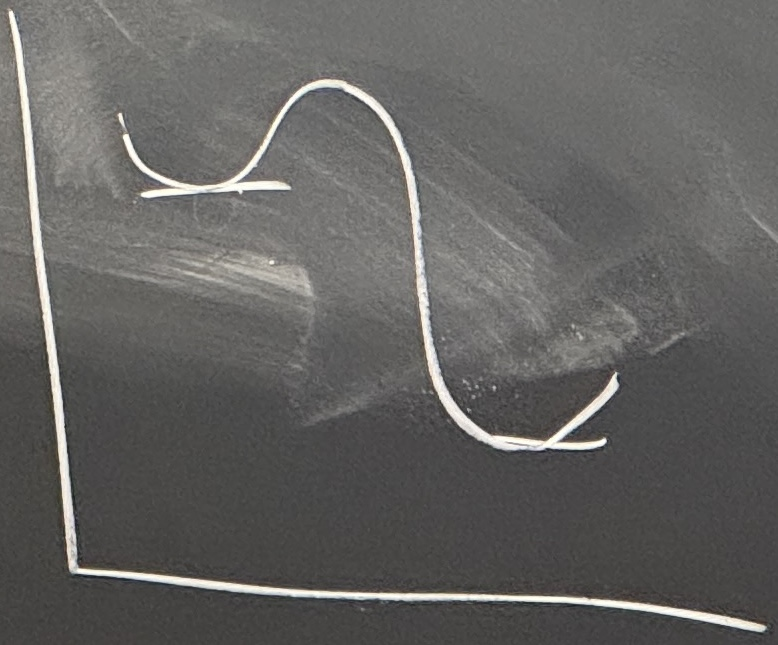
\includegraphics[width=0.55\linewidth]{mechAspectsb.JPG}
            \caption{Energy surface.}
            \label{fig:mechAspectsb}
        \end{subfigure}
        \begin{subfigure}[b]{0.3\linewidth}
            \centering
            \begin{equation*}
                \dv{\cnc{MeBr}}{t} = k\cnc{MeI}\cnc{Br-}
            \end{equation*}
            \caption{Kinetics.}
            \label{fig:mechAspectsc}
        \end{subfigure}
        \caption{Aspects of mechanism.}
        \label{fig:mechAspects}
    \end{figure}
    \begin{itemize}
        \item Three things we can consider in this mechanism are the orbital interactions, the potential energy surface along the reaction coordinate, and the kinetics.
    \end{itemize}
\end{itemize}




\end{document}